\batchmode
\nonstopmode
\documentclass[oneside]{article}
\n
% Packages required by doxygen
\usepackage{calc}
\usepackage{doxygen}
\usepackage{listings}
\usepackage{graphicx}
\usepackage[utf8]{inputenc}
\usepackage{makeidx}
\usepackage{multicol}
\usepackage{multirow}
\usepackage{textcomp}
\usepackage{amsmath}
\usepackage[table]{xcolor}
\usepackage{indentfirst}

% Font selection
\usepackage[T1]{fontenc}
\usepackage{mathptmx}
\usepackage[scaled=.90]{helvet}
\usepackage{courier}
\usepackage{amssymb}
\usepackage{sectsty}
\renewcommand{\familydefault}{\sfdefault}
\allsectionsfont{%
  \fontseries{bc}\selectfont%
  \color{darkgray}%
}
\renewcommand{\DoxyLabelFont}{%
  \fontseries{bc}\selectfont%
  \color{darkgray}%
}

% Page & text layout
\usepackage{geometry}
\geometry{%
  a4paper,%
  top=2.5cm,%
  bottom=2.5cm,%
  left=2.5cm,%
  right=2.5cm%
}
\tolerance=750
\hfuzz=15pt
\hbadness=750
\setlength{\emergencystretch}{15pt}
\setlength{\parindent}{0cm}
\setlength{\parskip}{0.2cm}
\makeatletter
\renewcommand{\paragraph}{%
  \@startsection{paragraph}{4}{0ex}{-1.0ex}{1.0ex}{%
\normalfont\normalsize\bfseries\SS@parafont%
  }%
}
\renewcommand{\subparagraph}{%
  \@startsection{subparagraph}{5}{0ex}{-1.0ex}{1.0ex}{%
\normalfont\normalsize\bfseries\SS@subparafont%
  }%
}
\makeatother

% Used by @code ... @endcode
\renewenvironment{DoxyCode}{%
  \par
  \normalsize
  \begin{alltt}%
}{%
  \end{alltt}%
  \normalsize%
}
% Headers & footers
\usepackage{fancyhdr}
\pagestyle{fancyplain}
\fancyhead[LE]{\fancyplain{}{\bfseries\thepage}}
\fancyhead[CE]{\fancyplain{}{}}
\fancyhead[RE]{\fancyplain{}{\bfseries\leftmark}}
\fancyhead[LO]{\fancyplain{}{\bfseries\rightmark}}
\fancyhead[CO]{\fancyplain{}{}}
\fancyhead[RO]{\fancyplain{}{\bfseries\thepage}}
\fancyfoot[LE]{\fancyplain{}{}}
\fancyfoot[CE]{\fancyplain{}{}}
\fancyfoot[RE]{\fancyplain{}{\bfseries\scriptsize PythonOCC User Guide - Topology and Geometry Modeling }}% : Topology and Geometry Modeling }}
\fancyfoot[LO]{\fancyplain{}{\bfseries\scriptsize PythonOCC User Guide - Topology and Geometry Modeling }}% : Topology and Geometry Modeling }
\fancyfoot[CO]{\fancyplain{}{}}
\fancyfoot[RO]{\fancyplain{}{}}
\renewcommand{\footrulewidth}{0.4pt}
\renewcommand{\sectionmark}[1]{%
  \markright{\thesection\ #1}%
}

% Indices & bibliography
\usepackage{natbib}
\usepackage[titles]{tocloft}
\renewcommand{\cftsecleader}{\cftdotfill{\cftdotsep}}
\setcounter{tocdepth}{3}
\setcounter{secnumdepth}{5}
\makeindex

% Hyperlinks (required, but should be loaded last)
\usepackage{ifpdf}
\ifpdf
  \usepackage[pdftex,pagebackref=true]{hyperref}
\else
  \usepackage[ps2pdf,pagebackref=true]{hyperref}
\fi
\hypersetup{%
  colorlinks=true,%
  linkcolor=black,%
  citecolor=black,%
  urlcolor=blue,%
  unicode%
}

% Custom commands
\newcommand{\clearemptydoublepage}{%
  \newpage{\pagestyle{empty}\cleardoublepage}%
}
\n


%===== C O N T E N T S =====\n
\begin{document}
% Titlepage & ToC
\hypersetup{pageanchor=false}
\pagenumbering{roman}
\begin{titlepage}
\vspace*{7cm}
\begin{center}%
\includegraphics[width=150px, height=150px]{../../../dox/resources/logo_pythonocc.png}\\
\vspace*{1cm}
{\Large PythonOCC 0.18.2 Documentation}\\
{\Large Topology and Geometry Modeling }\\
\vspace*{1cm}
{\small Thomas Paviot - \email{tpaviot@gmail.com}}\\
{\small originally written by the OpenCASCADE company}\\

\vspace*{1cm}
{\small Document version 0 - \today}\
\end{center}
\end{titlepage}
\clearpage
\pagenumbering{roman}
\tableofcontents
\newpage
\pagenumbering{arabic}
\hypersetup{pageanchor=true}

\let\stdsection\section
  \renewcommand\section{\pagebreak\stdsection}
\hypertarget{occt_user_guides__modeling_data}{}
\hypertarget{occt_user_guides__modeling_data_occt_modat_0}{}\section{Introduction}\label{occt_user_guides__modeling_data_occt_modat_0}
\hypertarget{occt_user_guides__modeling_data_label_about}{}\subsection{About this document}\label{occt_user_guides__modeling_data_label_about}
Modeling Data supplies data structures to represent 2D and 3D geometric models.\hypertarget{occt_user_guides__modeling_data_label_credits}{}\subsection{Credits and license}\label{occt_user_guides__modeling_data_label_credits}
This manual was originally written by the \href{http://www.opencascade.com}{\tt Open C\+A\+S\+C\+A\+DE company}. They\textquotesingle{}re the dev team that developed O\+CC Technology (O\+C\+CT), the underlying c++ layer on which Python\+O\+CC ia based.

This manual contains additions and modifications to fit with python specific syntax, and Python\+O\+CC usage in general. However, the basic concepts are the one available from O\+C\+CT. If you need further details related to O\+CC Technology, be aware that they offer commercial support and trainings, just check their \href{http://www.opencascade.com/content/tutorial-learning}{\tt E-\/learning \& Training} offerings. For your information, there is not any commercial agreement between the O\+CC Company and Python\+O\+CC development teams.

This document is distributed under the terms of the G\+NU Lesser General Public License (L\+G\+PL) version 2.\+1 with additional exception. Check the \href{https://github.com/tpaviot/PythonOCC-documentation/upstream_doc/LICENCES.md}{\tt license file} for more information.\hypertarget{occt_user_guides__modeling_data_label_resources}{}\subsection{Online resources}\label{occt_user_guides__modeling_data_label_resources}
If you need Python\+O\+CC specific help, please refer to the following online resources\+:


\begin{DoxyItemize}
\item Python\+O\+CC source code repository \href{https://github.com/tpaviot/PythonOCC-core}{\tt https\+://github.\+com/tpaviot/\+Python\+O\+C\+C-\/core}
\item Mailing list \href{http://groups.google.com/group/PythonOCC}{\tt http\+://groups.\+google.\+com/group/\+Python\+O\+CC}
\end{DoxyItemize}

Finally, email \{\href{mailto:tpaviot@gmail.com}{\tt tpaviot@gmail.\+com}\} for any other request.\hypertarget{occt_user_guides__modeling_data_typo}{}\subsection{Typographic conventions}\label{occt_user_guides__modeling_data_typo}
python code snippets use\+: lower\+\_\+case convention for variable names and functions, Camel\+Case for classes and methods. Example\+:


\begin{DoxyCode}
1 def create\_box(): \textcolor{comment}{# this is a function}
2   my\_box = BRepPrimAPI\_MakeBox(10, 20, 30) \textcolor{comment}{# a variable created from a Class}
3   \textcolor{keywordflow}{return} my\_box.Shape() \textcolor{comment}{# calling a .Method}
4 
5 a\_box\_shape = create\_box()
\end{DoxyCode}


In each code snippet, we assume that all required modules are loaded. For instance, in order to run the previous snippet, you have to import the B\+Rep\+Prim\+A\+P\+I\+\_\+\+Box class from the B\+Rep\+Prim\+A\+PI module just before\+:


\begin{DoxyCode}
1 \textcolor{keyword}{from} OCC.BRepPrimAPI \textcolor{keyword}{import} BRepPrimAPI\_MakeBox
\end{DoxyCode}
\hypertarget{occt_user_guides__modeling_data_improve}{}\subsection{Contribute improving this document}\label{occt_user_guides__modeling_data_improve}
The source code for this document is available in Doxygen mardkown format. Feel free to report issues, mistakes or submit patches using the issue tracker or pull request feature at\+:

\href{https://github.com/tpaviot/PythonOCC-documentation}{\tt https\+://github.\+com/tpaviot/\+Python\+O\+C\+C-\/documentation}.\hypertarget{occt_user_guides__modeling_data_occt_modat_5}{}\section{Topology}\label{occt_user_guides__modeling_data_occt_modat_5}
Python\+O\+CC Topology allows accessing and manipulating data of objects without dealing with their 2D or 3D representations. Whereas Python\+O\+CC Geometry provides a description of objects in terms of coordinates or parametric values, Topology describes data structures of objects in parametric space. These descriptions use location in and restriction of parts of this space.

Topological library allows you to build pure topological data structures. Topology defines relationships between simple geometric entities. In this way, you can model complex shapes as assemblies of simpler entities. Due to a built-\/in non-\/manifold (or mixed-\/dimensional) feature, you can build models mixing\+:
\begin{DoxyItemize}
\item 0D entities such as points,
\item 1D entities such as curves,
\item 2D entities such as surfaces,
\item 3D entities such as volumes.
\end{DoxyItemize}

You can, for example, represent a single object made of several distinct bodies containing embedded curves and surfaces connected or non-\/connected to an outer boundary.

Abstract topological data structure describes a basic entity -\/ a shape, which can be divided into the following component topologies\+:
\begin{DoxyItemize}
\item vertex -\/ a zero-\/dimensional shape corresponding to a point in geometry,
\item edge -\/ a shape corresponding to a curve, and bound by a vertex at each extremity,
\item wire -\/ a sequence of edges connected by their vertices,
\item face -\/ part of a plane (in 2D geometry) or a surface (in 3D geometry) bounded by a closed wire,
\item shell -\/ a collection of faces connected by some edges of their wire boundaries,
\item solid -\/ a part of 3D space bound by a shell,
\item compound solid -\/ a collection of solids.
\end{DoxyItemize}

The wire and the solid can be either infinite or closed.

A face with 3D underlying geometry may also refer to a collection of connected triangles that approximate the underlying surface. The surfaces can be undefined leaving the faces represented by triangles only. If so, the model is purely polyhedral.

Topology defines the relationship between simple geometric entities, which can thus be linked together to represent complex shapes.

Abstract Topology is provided by six modules. The first three modules describe the topological data structure used in Python\+O\+CC\+:


\begin{DoxyItemize}
\item {\itshape Top\+Abs} module provides general resources for topology-\/driven applications. It contains enumerations that are used to describe basic topological notions\+: topological shape, orientation and state. It also provides methods to manage these enumerations,
\item {\itshape Top\+Loc} module provides resources to handle 3D local coordinate systems\+: {\itshape Datum3\+D$\ast$and $\ast$\+Location}. {\itshape Datum3D} describes an elementary coordinate system, while {\itshape Location} comprises a series of elementary coordinate systems,
\item {\itshape Topo\+DS} module describes classes to model and build data structures that are purely topological.
\end{DoxyItemize}

Three additional modules provide tools to access and manipulate this abstract topology\+:


\begin{DoxyItemize}
\item {\itshape Top\+Tools} module provides basic tools to use on topological data structures,
\item {\itshape Top\+Exp} module provides classes to explore and manipulate the topological data structures described in the Topo\+DS module,
\item {\itshape B\+Rep\+Tools} module provides classes to explore, manipulate, read and write B\+Rep data structures. These more complex data structures combine topological descriptions with additional geometric information, and include rules for evaluating equivalence of different possible representations of the same object, for example, a point.
\end{DoxyItemize}\hypertarget{occt_user_guides__modeling_data_occt_modat_5_1}{}\subsection{Shape Location}\label{occt_user_guides__modeling_data_occt_modat_5_1}
A local coordinate system can be viewed as either of the following\+:
\begin{DoxyItemize}
\item a right-\/handed trihedron with an origin and three orthonormal vectors. The {\itshape gp\+\_\+\+Ax2} module corresponds to this definition,
\item a transformation of a +1 determinant, allowing the transformation of coordinates between local and global references frames. This corresponds to the {\itshape gp\+\_\+\+Trsf}.
\end{DoxyItemize}

{\itshape Top\+Loc} module distinguishes two notions\+:
\begin{DoxyItemize}
\item {\itshape Top\+Loc\+\_\+\+Datum3D} class provides the elementary reference coordinate, represented by a right-\/handed orthonormal system of axes or by a right-\/handed unitary transformation,
\item {\itshape Top\+Loc\+\_\+\+Location} class provides the composite reference coordinate made from elementary ones. It is a marker composed of a chain of references to elementary markers. The resulting cumulative transformation is stored in order to avoid recalculating the sum of the transformations for the whole list.
\end{DoxyItemize}


\begin{DoxyImage}
\begin{center}
 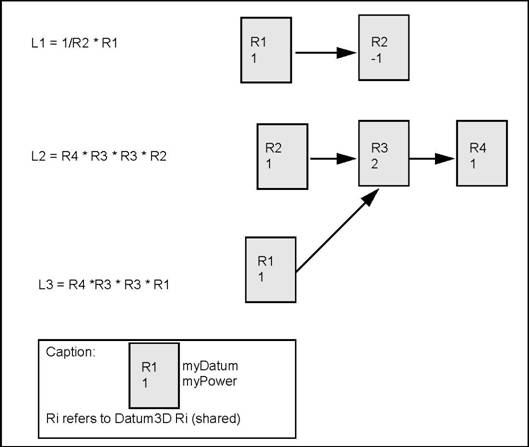
\includegraphics[width=\textwidth,height=\textheight/2,keepaspectratio=true]{modeling_data_image005.png}
\end{center}
\caption{Structure of Top\+Loc\+\_\+\+Location}
\end{DoxyImage}


Two reference coordinates are equal if they are made up of the same elementary coordinates in the same order. There is no numerical comparison. Two coordinates can thus correspond to the same transformation without being equal if they were not built from the same elementary coordinates.

For example, consider three elementary coordinates $R1, R2, R3$. The composite coordinates are\+:

$C1 = R1 \times R2$

$C2 = R2 \times R3$

$C3 = C1 \times R3$

$C4 = R1 \times C2$

{\bfseries N\+O\+TE} $C3$ and $C4$ are equal because they are both $R1 \times R2 \times R3$.

The {\itshape Top\+Loc} module is chiefly targeted at the topological data structure, but it can be used for other purposes.

\subsection*{Change of coordinates }

{\itshape Top\+Loc\+\_\+\+Datum3D} class represents a change of elementary coordinates. Such changes must be shared so this class inherits from {\itshape M\+Mgt\+\_\+\+T\+Shared}. The coordinate is represented by a transformation {\itshape gp\+\_\+\+Trsfmodule}. This transformation has no scaling factor.\hypertarget{occt_user_guides__modeling_data_occt_modat_5_2}{}\subsection{Naming shapes, sub-\/shapes, their orientation and state}\label{occt_user_guides__modeling_data_occt_modat_5_2}
The {\itshape Top\+Abs} module provides general enumerations describing the basic concepts of topology and methods to handle these enumerations. It contains no classes. This module has been separated from the rest of the topology because the notions it contains are sufficiently general to be used by all topological tools. This avoids redefinition of enumerations by remaining independent of modeling resources. The Top\+Abs module defines three notions\+:
\begin{DoxyItemize}
\item the shape type\+: {\itshape Top\+Abs\+\_\+\+Shape\+Enum},
\item the shape orientation\+: {\itshape Top\+Abs\+\_\+\+Orientation},
\item the shape state\+: {\itshape State\+Top\+Abs\+\_\+\+State} .
\end{DoxyItemize}\hypertarget{occt_user_guides__modeling_data_occt_modat_5_2_1}{}\subsubsection{Topological types}\label{occt_user_guides__modeling_data_occt_modat_5_2_1}
Top\+Abs contains the {\itshape Top\+Abs\+\_\+\+Shape\+Enum} enumeration,which lists the different topological types\+:
\begin{DoxyItemize}
\item Top\+Abs\+\_\+\+C\+O\+M\+P\+O\+U\+ND\+: a group of any type of topological objects,
\item Top\+Abs\+\_\+\+C\+O\+M\+P\+S\+O\+L\+ID\+: a composite solid is a set of solids connected by their faces. It expands the notions of W\+I\+RE and S\+H\+E\+LL to solids,
\item Top\+Abs\+\_\+\+S\+O\+L\+ID\+: a part of space limited by shells. It is three dimensional,
\item Top\+Abs\+\_\+\+S\+H\+E\+LL\+: a set of faces connected by their edges. A shell can be open or closed,
\item Top\+Abs\+\_\+\+F\+A\+CE\+: in 2D it is a part of a plane; in 3D it is a part of a surface. Its geometry is constrained (trimmed) by contours. It is two dimensional,
\item Top\+Abs\+\_\+\+W\+I\+RE\+: a set of edges connected by their vertices. It can be an open or closed contour depending on whether the edges are linked or not,
\item Top\+Abs\+\_\+\+E\+D\+GE\+: a topological element corresponding to a restrained curve. An edge is generally limited by vertices. It has one dimension,
\item Top\+Abs\+\_\+\+V\+E\+R\+T\+EX\+: a topological element corresponding to a point. It has zero dimension,
\item Top\+Abs\+\_\+\+S\+H\+A\+PE\+: a generic term covering all of the above.
\end{DoxyItemize}

A topological model can be considered as a graph of objects with adjacency relationships. When modeling a part in 2D or 3D space it must belong to one of the categories listed in the Shape\+Enum enumeration. The Top\+Absmodule lists all the objects, which can be found in any model. It cannot be extended but a subset can be used. For example, the notion of solid is useless in 2D.

The terms of the enumeration appear in order from the most complex to the most simple, because objects can contain simpler objects in their description. For example, a face references its wires, edges, and vertices. 
\begin{DoxyImage}
\begin{center}
 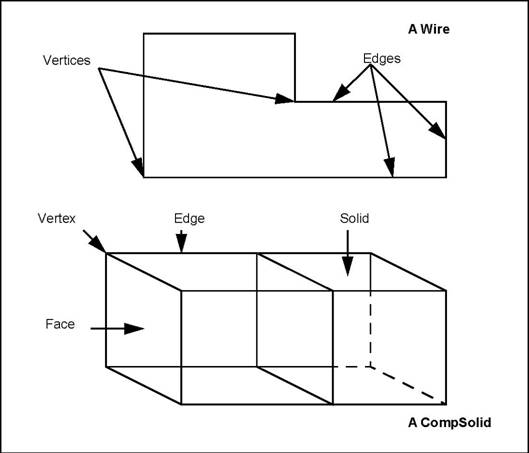
\includegraphics[width=\textwidth,height=\textheight/2,keepaspectratio=true]{modeling_data_image006.png}
\end{center}
\caption{Shape\+Enum}
\end{DoxyImage}
 \hypertarget{occt_user_guides__modeling_data_occt_modat_5_2_2}{}\subsubsection{Orientation}\label{occt_user_guides__modeling_data_occt_modat_5_2_2}
The notion of orientation is represented by the {\itshape Top\+Abs\+\_\+\+Orientation} enumeration. Orientation is a generalized notion of the sense of direction found in various modelers. This is used when a shape limits a geometric domain; and is closely linked to the notion of boundary. The three cases are the following\+:
\begin{DoxyItemize}
\item curve limited by a vertex,
\item surface limited by an edge,
\item space limited by a face.
\end{DoxyItemize}

In each case the topological form used as the boundary of a geometric domain of a higher dimension defines two local regions of which one is arbitrarily considered as the {\itshape default region}.

For a curve limited by a vertex the default region is the set of points with parameters greater than the vertex. That is to say it is the part of the curve after the vertex following the natural direction along the curve.

For a surface limited by an edge the default region is on the left of the edge following its natural direction. More precisely it is the region pointed to by the vector product of the normal vector to the surface and the vector tangent to the curve.

For a space limited by a face the default region is found on the negative side of the normal to the surface.

Based on this default region the orientation allows definition of the region to be kept, which is called the {\itshape interior} or {\itshape material}. There are four orientations defining the interior.

\tabulinesep=1mm
\begin{longtabu} spread 0pt [c]{*2{|X[-1]}|}
\hline
\rowcolor{\tableheadbgcolor}{\bf Orientation }&{\bf Description  }\\\cline{1-2}
\endfirsthead
\hline
\endfoot
\hline
\rowcolor{\tableheadbgcolor}{\bf Orientation }&{\bf Description  }\\\cline{1-2}
\endhead
Top\+Abs\+\_\+\+F\+O\+R\+W\+A\+RD &The interior is the default region. \\\cline{1-2}
Top\+Abs\+\_\+\+R\+E\+V\+E\+R\+S\+ED &The interior is the region complementary to the default. \\\cline{1-2}
Top\+Abs\+\_\+\+I\+N\+T\+E\+R\+N\+AL &The interior includes both regions. The boundary lies inside the material. For example a surface inside a solid. \\\cline{1-2}
Top\+Abs\+\_\+\+E\+X\+T\+E\+R\+N\+AL &The interior includes neither region. The boundary lies outside the material. For example an edge in a wire-\/frame model. \\\cline{1-2}
\end{longtabu}

\begin{DoxyImage}
\begin{center}
 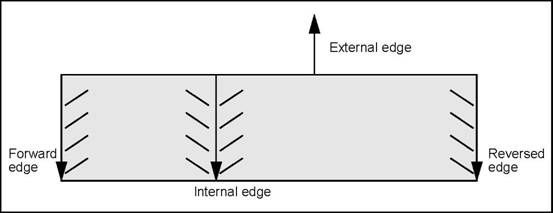
\includegraphics[width=\textwidth,height=\textheight/2,keepaspectratio=true]{modeling_data_image007.png}
\end{center}
\caption{Four Orientations}
\end{DoxyImage}


The notion of orientation is a very general one, and it can be used in any context where regions or boundaries appear. Thus, for example, when describing the intersection of an edge and a contour it is possible to describe not only the vertex of intersection but also how the edge crosses the contour considering it as a boundary. The edge would therefore be divided into two regions -\/ exterior and interior -\/ with the intersection vertex as the boundary. Thus an orientation can be associated with an intersection vertex as in the following figure\+:

\tabulinesep=1mm
\begin{longtabu} spread 0pt [c]{*2{|X[-1]}|}
\hline
\rowcolor{\tableheadbgcolor}{\bf Orientation }&{\bf Association  }\\\cline{1-2}
\endfirsthead
\hline
\endfoot
\hline
\rowcolor{\tableheadbgcolor}{\bf Orientation }&{\bf Association  }\\\cline{1-2}
\endhead
Top\+Abs\+\_\+\+F\+O\+R\+W\+A\+RD &Entering \\\cline{1-2}
Top\+Abs\+\_\+\+R\+E\+V\+E\+R\+S\+ED &Exiting \\\cline{1-2}
Top\+Abs\+\_\+\+I\+N\+T\+E\+R\+N\+AL &Touching from inside \\\cline{1-2}
Top\+Abs\+\_\+\+E\+X\+T\+E\+R\+N\+AL &Touching from outside \\\cline{1-2}
\end{longtabu}

\begin{DoxyImage}
\begin{center}
 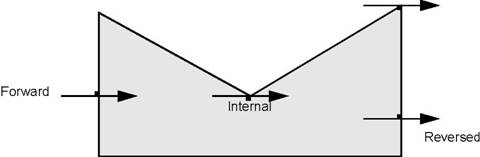
\includegraphics[width=\textwidth,height=\textheight/2,keepaspectratio=true]{modeling_data_image008.png}
\end{center}
\caption{Four orientations of intersection vertices}
\end{DoxyImage}


Along with the Orientation enumeration the {\itshape Top\+Abs} module defines four methods\+:


\begin{DoxyItemize}
\item {\itshape topabs\+\_\+\+Complement},
\item {\itshape topabs\+\_\+\+Compose},
\item {\itshape topabs\+\_\+\+Print},
\item {\itshape topabs\+\_\+\+Reverse}.
\end{DoxyItemize}\hypertarget{occt_user_guides__modeling_data_occt_modat_5_2_3}{}\subsubsection{State}\label{occt_user_guides__modeling_data_occt_modat_5_2_3}
The {\itshape Top\+Abs\+\_\+\+State} enumeration described the position of a vertex or a set of vertices with respect to a region. There are four terms\+:

\tabulinesep=1mm
\begin{longtabu} spread 0pt [c]{*2{|X[-1]}|}
\hline
\rowcolor{\tableheadbgcolor}{\bf Position }&{\bf Description  }\\\cline{1-2}
\endfirsthead
\hline
\endfoot
\hline
\rowcolor{\tableheadbgcolor}{\bf Position }&{\bf Description  }\\\cline{1-2}
\endhead
Top\+Abs\+\_\+\+IN &The point is interior. \\\cline{1-2}
Top\+Abs\+\_\+\+O\+UT &The point is exterior. \\\cline{1-2}
Top\+Abs\+\_\+\+ON &The point is on the boundary(within tolerance). \\\cline{1-2}
Top\+Abs\+\_\+\+U\+N\+K\+N\+O\+WN &The state of the point is indeterminate. \\\cline{1-2}
\end{longtabu}
The U\+N\+K\+N\+O\+WN term has been introduced because this enumeration is often used to express the result of a calculation, which can fail. This term can be used when it is impossible to know if a point is inside or outside, which is the case with an open wire or face.


\begin{DoxyImage}
\begin{center}
 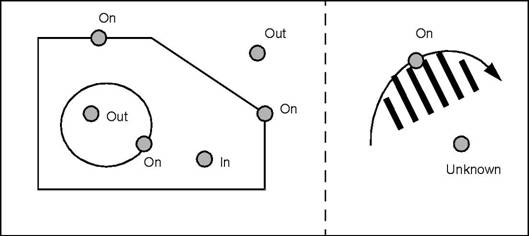
\includegraphics[width=\textwidth,height=\textheight/2,keepaspectratio=true]{modeling_data_image009.png}
\end{center}
\caption{The four states}
\end{DoxyImage}


The State enumeration can also be used to specify various parts of an object. The following figure shows the parts of an edge intersecting a face.


\begin{DoxyImage}
\begin{center}
 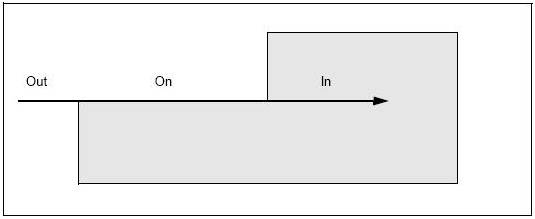
\includegraphics[width=\textwidth,height=\textheight/2,keepaspectratio=true]{modeling_data_image010.png}
\end{center}
\caption{State specifies the parts of an edge intersecting a face}
\end{DoxyImage}
\hypertarget{occt_user_guides__modeling_data_occt_modat_5_3}{}\subsection{Manipulating shapes and sub-\/shapes}\label{occt_user_guides__modeling_data_occt_modat_5_3}
The {\itshape Topo\+DS} module describes the topological data structure with the following characteristics\+:
\begin{DoxyItemize}
\item reference to an abstract shape with neither orientation nor location,
\item access to the data structure through the tool classes.
\end{DoxyItemize}

As stated above, Python\+O\+CC Topology describes data structures of objects in parametric space. These descriptions use localization in and restriction of parts of this space. The types of shapes, which can be described in these terms, are the vertex, the face and the shape. The vertex is defined in terms of localization in parametric space, and the face and shape, in terms of restriction of this space.

Python\+O\+CC topological descriptions also allow the simple shapes defined in these terms to be combined into sets. For example, a set of edges forms a wire; a set of faces forms a shell, and a set of solids forms a composite solid (Comp\+Solid in Python\+O\+CC). You can also combine shapes of either sort into compounds. Finally, you can give a shape an orientation and a location.

Listing shapes in order of complexity from vertex to composite solid leads us to the notion of the data structure as knowledge of how to break a shape down into a set of simpler shapes. This is in fact, the purpose of the {\itshape Topo\+DS} module.

The model of a shape is a shareable data structure because it can be used by other shapes. (An edge can be used by more than one face of a solid). A shareable data structure is handled by reference. When a simple reference is insufficient, two pieces of information are added -\/ an orientation and a local coordinate reference.
\begin{DoxyItemize}
\item an orientation tells how the referenced shape is used in a boundary ({\itshape Top\+Abs\+\_\+\+Orientation}),
\item a local reference coordinate ({\itshape Top\+Loc\+\_\+\+Location}) allows referencing a shape at a position different from that of its definition.
\end{DoxyItemize}

The {\itshape Topo\+D\+S\+\_\+\+T\+Shape} class is the root of all shape descriptions. It contains a list of shapes. Classes inheriting {\itshape Topo\+D\+S\+\_\+\+T\+Shape} can carry the description of a geometric domain if necessary (for example, a geometric point associated with a T\+Vertex). A {\itshape Topo\+D\+S\+\_\+\+T\+Shape} is a description of a shape in its definition frame of reference. This class is manipulated by reference.

The {\itshape Topo\+D\+S\+\_\+\+Shape} class describes a reference to a shape. It contains a reference to an underlying abstract shape, an orientation,and a local reference coordinate. This class is manipulated by value and thus cannot be shared.

The class representing the underlying abstract shape is never referenced directly. The {\itshape Topo\+D\+S\+\_\+\+Shape} class is always used to refer to it.

The information specific to each shape (the geometric support) is always added by inheritance to classes deriving from {\itshape Topo\+D\+S\+\_\+\+T\+Shape}. The following figures show the example of a shell formed from two faces connected by an edge.


\begin{DoxyImage}
\begin{center}
 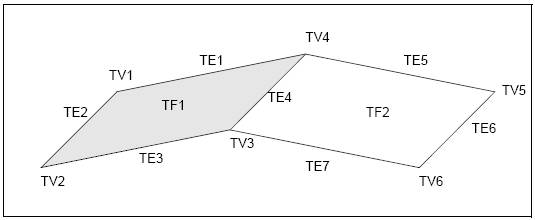
\includegraphics[width=\textwidth,height=\textheight/2,keepaspectratio=true]{modeling_data_image011.png}
\end{center}
\caption{Structure of a shell formed from two faces}
\end{DoxyImage}



\begin{DoxyImage}
\begin{center}
 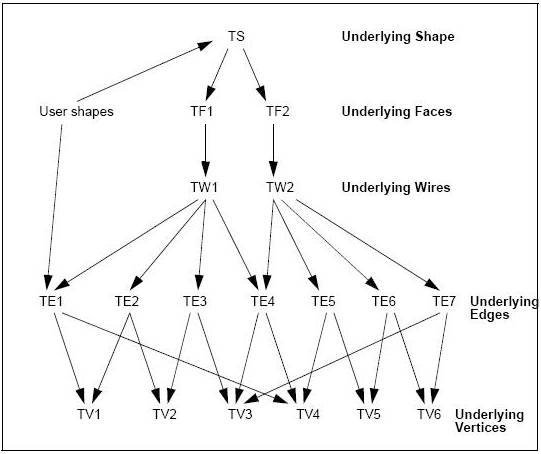
\includegraphics[width=\textwidth,height=\textheight/2,keepaspectratio=true]{modeling_data_image012.png}
\end{center}
\caption{Data structure of the above shell}
\end{DoxyImage}


In the previous diagram, the shell is described by the underlying shape TS, and the faces by T\+F1 and T\+F2. There are seven edges from T\+E1 to T\+E7 and six vertices from T\+V1 to T\+V6.

The wire T\+W1 references the edges from T\+E1 to T\+E4; T\+W2 references from T\+E4 to T\+E7.

The vertices are referenced by the edges as follows\+:T\+E1(\+T\+V1,\+T\+V4), T\+E2(\+T\+V1,\+T\+V2), T\+E3(\+T\+V2,\+T\+V3), T\+E4(\+T\+V3,\+T\+V4), T\+E5(\+T\+V4,\+T\+V5), T\+E6(\+T5,\+T\+V6),T\+E7(\+T\+V3,\+T\+V6).

{\bfseries Note}\+: this data structure does not contain any {\itshape back references}. All references go from more complex underlying shapes to less complex ones. The techniques used to access the information are described later. The data structure is as compact as possible. Sub-\/objects can be shared among different objects.

Two very similar objects, perhaps two versions of the same object, might share identical sub-\/objects. The usage of local coordinates in the data structure allows the description of a repetitive sub-\/structure to be shared.

The compact data structure avoids the loss of information associated with copy operations which are usually used in creating a new version of an object or when applying a coordinate change.

The following figure shows a data structure containing two versions of a solid. The second version presents a series of identical holes bored at different positions. The data structure is compact and yet keeps all information on the sub-\/elements.

The three references from {\itshape T\+Sh2} to the underlying face {\itshape T\+Fcyl} have associated local coordinate systems, which correspond to the successive positions of the hole. 
\begin{DoxyImage}
\begin{center}
 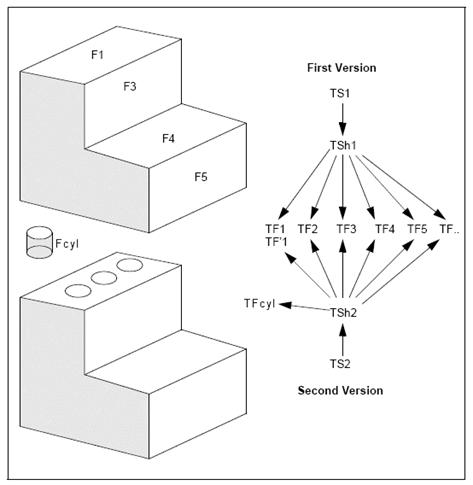
\includegraphics[width=\textwidth,height=\textheight/2,keepaspectratio=true]{modeling_data_image013.png}
\end{center}
\caption{Data structure containing two versions of a solid}
\end{DoxyImage}


\subsection*{Classes inheriting Topo\+D\+S\+\_\+\+Shape }

{\itshape Topo\+DS} is based on class {\itshape Topo\+D\+S\+\_\+\+Shape} and the class defining its underlying shape. This has certain advantages, but the major drawback is that these classes are too general. Different shapes they could represent do not type them (Vertex, Edge, etc.) hence it is impossible to introduce checks to avoid incoherences such as inserting a face in an edge.

{\itshape Topo\+DS} module offers two sets of classes, one set inheriting the underlying shape with neither orientation nor location and the other inheriting {\itshape Topo\+D\+S\+\_\+\+Shape}, which represent the standard topological shapes enumerated in {\itshape Top\+Abs} module.

The following classes inherit from {\itshape Topo\+D\+S\+\_\+\+Shape} \+: {\itshape Topo\+D\+S\+\_\+\+Vertex, Topo\+D\+S\+\_\+\+Edge, Topo\+D\+S\+\_\+\+Wire, Topo\+D\+S\+\_\+\+Face, Topo\+D\+S\+\_\+\+Shell, Topo\+D\+S\+\_\+\+Solid,Topo\+D\+S\+\_\+\+Comp\+Solid,} and {\itshape Topo\+D\+S\+\_\+\+Compound}. In spite of the similarity of names with those inheriting from {\itshape Topo\+D\+S\+\_\+\+T\+Shape} there is a profound difference in the way they are used.

{\itshape Topo\+D\+S\+\_\+\+Shape} class and the classes, which inherit from it, are the natural means to manipulate topological objects. {\itshape Topo\+D\+S\+\_\+\+T\+Shape} classes are hidden. {\itshape Topo\+D\+S\+\_\+\+T\+Shape} describes a class in its original local coordinate system without orientation. {\itshape Topo\+D\+S\+\_\+\+Shape} is a reference to {\itshape Topo\+D\+S\+\_\+\+T\+Shape} with an orientation and a local reference.

{\itshape Topo\+D\+S\+\_\+\+T\+Shape} class is deferred; {\itshape Topo\+D\+S\+\_\+\+Shape} class is not. Using {\itshape Topo\+D\+S\+\_\+\+Shape} class allows manipulation of topological objects without knowing their type. It is a generic form. Purely topological algorithms often use the {\itshape Topo\+D\+S\+\_\+\+Shape} class.

{\itshape Topo\+D\+S\+\_\+\+T\+Shape} class is manipulated by reference; Topo\+D\+S\+\_\+\+Shape class by value. A Topo\+D\+S\+\_\+\+Shape is nothing more than a reference enhanced with an orientation and a local coordinate. The sharing of {\itshape Topo\+D\+S\+\_\+\+Shapes} is meaningless. What is important is the sharing of the underlying {\itshape Topo\+D\+S\+\_\+\+T\+Shapes}. Assignment or passage in argument does not copy the data structure\+: this only creates new {\itshape Topo\+D\+S\+\_\+\+Shapes} which refer to the same {\itshape Topo\+D\+S\+\_\+\+T\+Shape}.

Although classes inheriting {\itshape Topo\+D\+S\+\_\+\+T\+Shape} are used for adding extra information, extra fields should not be added in a class inheriting from Topo\+D\+S\+\_\+\+Shape. Classes inheriting from Topo\+D\+S\+\_\+\+Shape serve only to specialize a reference in order to benefit from static type control (carried out by the compiler). For example, a routine that receives a {\itshape Topo\+D\+S\+\_\+\+Face} in argument is more precise for the compiler than the one, which receives a {\itshape Topo\+D\+S\+\_\+\+Shape}. It is pointless to derive other classes than those found in\+Topo\+DS. All references to a topological data structure are made with the Shape class and its inheritors defined in {\itshape Topo\+DS}.

There are no constructors for the classes inheriting from the {\itshape Topo\+D\+S\+\_\+\+Shape} class, otherwise the type control would disappear through {\bfseries implicit casting} (a characteristic of C++). The Topo\+DS module provides module methods for {\bfseries casting} an object of the Topo\+D\+S\+\_\+\+Shape class in one of these sub-\/classes, with type verification.

The following example shows a routine receiving an argument of the {\itshape Topo\+D\+S\+\_\+\+Shape} type, then putting it into a variable V if it is a vertex or calling the method Process\+Edge if it is an edge.


\begin{DoxyCode}
1 \textcolor{keyword}{from} OCC.Core.TopAbs \textcolor{keyword}{import} TopAbs\_VERTEX, TopAbs\_Edge
2 \textcolor{keyword}{from} OCC.Core.TopoDS \textcolor{keyword}{import} topods\_Vertex, topods\_Edge
3 
4 \textcolor{keyword}{def }process\_edge(an\_edge):
5   \textcolor{stringliteral}{""" an\_edge : a TopoDS\_Edge}
6 \textcolor{stringliteral}{  """}
7   ... do something 
8 
9 \textcolor{keyword}{def }process(a\_shape):
10   \textcolor{stringliteral}{""" a\_shape : TopoDS\_Shape}
11 \textcolor{stringliteral}{  """}  
12   \textcolor{keywordflow}{if} aShape.Shapetype() == TopAbs\_VERTEX:
13     v = topods\_Vertex(aShape)
14   \textcolor{keywordflow}{elif} aShape.ShapeType() == TopAbs\_EDGE:
15     e topods\_Edge(a\_shape)
16     process\_edge(e)
17   \textcolor{keywordflow}{else}:
18     print(\textcolor{stringliteral}{"Neither a vertex nor an edge."})
\end{DoxyCode}
\hypertarget{occt_user_guides__modeling_data_occt_modat_5_4}{}\subsection{Exploration of Topological Data Structures}\label{occt_user_guides__modeling_data_occt_modat_5_4}
The {\itshape Top\+Exp} module provides tools for exploring the data structure described with the {\itshape Topo\+DS} module. Exploring a topological structure means finding all sub-\/objects of a given type, for example, finding all the faces of a solid.

The Top\+Exp module provides the class {\itshape Top\+Exp\+\_\+\+Explorer} to find all sub-\/objects of a given type. An explorer is built with\+:
\begin{DoxyItemize}
\item the shape to be explored,
\item the type of shapes to be found e.\+g. {\itshape Top\+Abs\+\_\+\+V\+E\+R\+T\+EX}, {\itshape Top\+Abs\+\_\+\+E\+D\+GE} with the exception of {\itshape Top\+Abs\+\_\+\+S\+H\+A\+PE}, which is not allowed,
\item the type of Shapes to avoid. e.\+g. {\itshape Top\+Abs\+\_\+\+S\+H\+E\+LL}, {\itshape Top\+Abs\+\_\+\+E\+D\+GE}. By default, this type is {\itshape Top\+Abs\+\_\+\+S\+H\+A\+PE}. This default value means that there is no restriction on the exploration.
\end{DoxyItemize}

The {\itshape Top\+Exp\+\_\+\+Explorer} class visits the whole structure in order to find the shapes of the requested type not contained in the type to avoid. The example below shows how to find all faces in the shape {\itshape S}\+:


\begin{DoxyCode}
1 \textcolor{keyword}{from} OCC.Core.TopExp \textcolor{keyword}{import} TopExp\_Explorer
2 
3 \textcolor{keyword}{def }process\_face(a\_topods\_shape):
4   ... \textcolor{comment}{## anything that takes and processes a TopoDS\_Face}
5 
6 \textcolor{keyword}{def }test():
7   shp = ... \textcolor{comment}{# any TopoDS\_Shape }
8   exp = TopExp\_Explorer()
9   exp.Init(shp, TopAbs\_FACE)
10   \textcolor{keywordflow}{while} exp.More():
11     process\_face(exp.Current())
12     exp.Next()
\end{DoxyCode}


Find all the vertices which are not in an edge


\begin{DoxyCode}
1 exp.Init(shp, TopAbs\_VERTEX, TopAbs\_EDGE)
\end{DoxyCode}


Find all the faces in a S\+H\+E\+LL, then all the faces not in a S\+H\+E\+LL\+:


\begin{DoxyCode}
1 \textcolor{keyword}{def }test():
2   shp = ... \textcolor{comment}{## any TopoDS\_Shape}
3   exp1 = TopExp\_Explorer()
4   exp2 = TopExp\_Explorer()
5   exp1.Init(shp, TopAbs\_SHELL)
6   \textcolor{keywordflow}{while} exp1.More():
7     exp1.Next() 
8     \textcolor{comment}{# visit all shells}
9     exp2.Init(exp1.Current()
10     \textcolor{keywordflow}{while} exp2.More():
11      \textcolor{comment}{# visit all the faces of the current shell }
12      ProcessFaceinAshell(exp2.Current())
13      exp2.Next()
14     exp1.Next()
15   exp1.Init(shp, TopAbs\_FACE, TopAbs\_SHELL)
16   \textcolor{keywordflow}{while} exp1.More():
17     \textcolor{comment}{# visit all faces not ina shell. }
18     process\_face(exp.Current())
19     exp1.Next()
\end{DoxyCode}


The Explorer presumes that objects contain only objects of an equal or inferior type. For example, if searching for faces it does not look at wires, edges, or vertices to see if they contain faces.

The {\itshape Map\+Shapes} method from the {\itshape topexp} class allows filling a Map. An exploration using the {\itshape Top\+Exp\+\_\+\+Explorer} class can visit an object more than once if it is referenced more than once. For example, an edge of a solid is generally referenced by two faces. To process objects only once, they have to be placed in a Map.\hypertarget{occt_user_guides__modeling_data_occt_modat_5_5}{}\subsection{Lists and Maps of Shapes}\label{occt_user_guides__modeling_data_occt_modat_5_5}
{\itshape Top\+Tools} module contains tools for exploiting the {\itshape Topo\+DS} data structure. It is an instantiation of the tools from {\itshape T\+Collection} module with the Shape classes of {\itshape Topo\+DS}.


\begin{DoxyItemize}
\item {\itshape Top\+Tools\+\_\+\+Array1\+Of\+Shape, H\+Array1\+Of\+Shape} -\/ Instantiation of the {\itshape T\+Collection\+\_\+\+Array1} and {\itshape T\+Collection\+\_\+\+H\+Array1} with {\itshape Topo\+D\+S\+\_\+\+Shape},
\item {\itshape Top\+Tools\+\_\+\+Sequence\+Of\+Shape} -\/ Instantiation of the {\itshape T\+Collection\+\_\+\+Sequence} with {\itshape Topo\+D\+S\+\_\+\+Shape},
\item {\itshape Top\+Tools\+\_\+\+Map\+Of\+Shape} -\/ Instantiation of the {\itshape T\+Collection\+\_\+\+Map}. Allows the construction of sets of shapes,
\item {\itshape Top\+Tools\+\_\+\+Indexed\+Map\+Of\+Shape} -\/ Instantiation of the {\itshape T\+Collection\+\_\+\+Indexed\+Map}. Allows the construction of tables of shapes and other data structures.
\end{DoxyItemize}

With a {\itshape Top\+Tools\+\_\+\+Map}, a set of references to Shapes can be kept without duplication. The following example counts the size of a data structure as a number of {\itshape T\+Shapes}.


\begin{DoxyCode}
1 \textcolor{keyword}{def }get\_shape\_size(a\_shp):
2   \textcolor{stringliteral}{""" returns the size of a shape.}
3 \textcolor{stringliteral}{  This is a recursive method. }
4 \textcolor{stringliteral}{  The size of a shape is1 + the sizes of the subshapes. }
5 \textcolor{stringliteral}{}
6 \textcolor{stringliteral}{  a\_shp : a TopoDS\_Shape}
7 \textcolor{stringliteral}{  """}
8   it = TopoDS\_Iterator()
9   it.Initialize(a\_shp)
10   size = 1 
11   \textcolor{keywordflow}{while} it.More():
12    size += get\_shape\_size(it.Value())
13    it.Next()
14  \textcolor{keywordflow}{return} size
\end{DoxyCode}


This program is incorrect if there is sharing in the data structure.

Thus for a contour of four edges it should count 1 wire + 4 edges +4 vertices with the result 9, but as the vertices are each shared by two edges this program will return 13. One solution is to put all the Shapes in a Map so as to avoid counting them twice, as in the following example\+:


\begin{DoxyCode}
1 \textcolor{keyword}{def }map\_shapes(a\_shape, a\_map):
2  \textcolor{stringliteral}{"""}
3 \textcolor{stringliteral}{ a\_shape: a TopoDS\_Shape}
4 \textcolor{stringliteral}{ a\_map: a TopTools\_MapOfShape}
5 \textcolor{stringliteral}{ """}
6  \textcolor{comment}{# This is a recursive auxiliary method. It stores all subShapes of aShape in a Map.}
7  \textcolor{keywordflow}{if} a\_map.Add(a\_shape):
8    \textcolor{comment}{## Add returns True if aShape was not already in the Map. }
9    it = TopoDS\_Iterator()
10    it.Initiliaze(a\_shape)
11    \textcolor{keywordflow}{while} it.More():
12      map\_shapes(it.Value(), a\_map)
13      it.Next()
14 
15 
16 \textcolor{keyword}{def }size(a\_shape):
17   \textcolor{stringliteral}{"""}
18 \textcolor{stringliteral}{  a\_shape: a TopoDS\_Shape}
19 \textcolor{stringliteral}{  """}
20   \textcolor{comment}{# Store Shapes in a Mapand return the size. }
21   m = TopTools\_MapOfShape()
22   map\_shapes(a\_shape, m)
23   \textcolor{keywordflow}{return} m.Extent()
24 
25 
26 sh = ... \textcolor{comment}{# any TopoDS\_Shape}
27 print(size(sh))
\end{DoxyCode}


The following example is more ambitious and writes a program which copies a data structure using an {\itshape Top\+Tools\+\_\+\+Indexed\+Map}. The copy is an identical structure but it shares nothing with the original. The principal algorithm is as follows\+:
\begin{DoxyItemize}
\item all Topo\+D\+S\+\_\+\+Shape instances in the structure are put into an {\itshape Top\+Tools\+\_\+\+Indexed\+Map},
\item a table of Topo\+D\+S\+\_\+\+Shape instances is created in parallel with the map to receive the copies,
\item the structure is copied using the auxiliary recursive function, which copies from the map to the array.
\end{DoxyItemize}


\begin{DoxyCode}
1 \textcolor{keyword}{def }copy(a\_shape, a\_builder):
2  \textcolor{stringliteral}{"""" aShape: a TopoDS\_Shape instance}
3 \textcolor{stringliteral}{ a\_builder: a TopoDS\_Builder instance}
4 \textcolor{stringliteral}{ Returns a TopoDS\_Shape}
5 \textcolor{stringliteral}{ """}
6  \textcolor{comment}{# Copies the wholestructure of a\_shape using a\_builder. }
7  \textcolor{comment}{# Stores all the sub-Shapes in an IndexedMap. }
8  theMap = TopTools\_IndexedMapOfShape()
9  it = TopoDS\_Iterator()
10  theMap.Add(a\_shape)
11  \textcolor{keywordflow}{for} i \textcolor{keywordflow}{in} range(1, theMap.Extent()):
12   it.Initialize(theMap(i))
13   \textcolor{keywordflow}{while} it.More():
14     s=It.Value()
15     s.Location(Identity)
16     s.Orientation(TopAbs\_FORWARD)
17     theMap.Add(s) 
18     it.Next()
\end{DoxyCode}
\hypertarget{occt_user_guides__modeling_data_occt_modat_5_5_1}{}\subsubsection{Wire Explorer}\label{occt_user_guides__modeling_data_occt_modat_5_5_1}
{\itshape B\+Rep\+Tools\+\_\+\+Wire\+Explorer} class can access edges of a wire in their order of connection.

For example, in the wire in the image we want to recuperate the edges in the order \{e1, e2, e3,e4, e5\} \+:


\begin{DoxyImage}
\begin{center}
 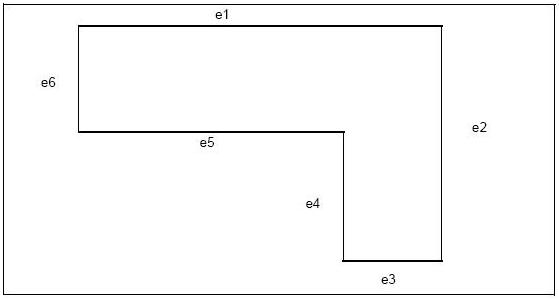
\includegraphics[width=\textwidth,height=\textheight/2,keepaspectratio=true]{modeling_data_image014.png}
\end{center}
\caption{A wire composed of 6 edges.}
\end{DoxyImage}


{\itshape Top\+Exp\+\_\+\+Explorer}, however, recuperates the lines in any order.


\begin{DoxyCode}
1 w = ... \textcolor{comment}{# any TopoDS\_Wire}
2 ex = BRepTools\_WireExplorer()
3 ex.Init(w)
4 \textcolor{keywordflow}{while} ex.More():
5  process\_current\_endge(ex.Current())
6  \textcolor{comment}{# ProcessTheVertexConnectingTheCurrentEdgeToThePrevious }
7  one(ex.CurrentVertex())
8  ex.Next() 
\end{DoxyCode}
\hypertarget{occt_user_guides__modeling_data_occt_modat_1}{}\section{Geometry Utilities}\label{occt_user_guides__modeling_data_occt_modat_1}
Geometry Utilities provide the following services\+:
\begin{DoxyItemize}
\item creation of shapes by interpolation and approximation,
\item direct construction of shapes,
\item conversion of curves and surfaces to B\+Spline curves and surfaces,
\item computation of the coordinates of points on 2D and 3D curves,
\item calculation of extrema between shapes.
\end{DoxyItemize}\hypertarget{occt_user_guides__modeling_data_occt_modat_1_1}{}\subsection{Interpolations and Approximations}\label{occt_user_guides__modeling_data_occt_modat_1_1}
In modeling, it is often required to approximate or interpolate points into curves and surfaces. In interpolation, the process is complete when the curve or surface passes through all the points; in approximation, when it is as close to these points as possible.

Approximation of Curves and Surfaces groups together a variety of functions used in 2D and 3D geometry for\+:
\begin{DoxyItemize}
\item the interpolation of a set of 2D points using a 2D B\+Spline or Bezier curve,
\item the approximation of a set of 2D points using a 2D B\+Spline or Bezier curve,
\item the interpolation of a set of 3D points using a 3D B\+Spline or Bezier curve, or a B\+Spline surface,
\item the approximation of a set of 3D points using a 3D B\+Spline or Bezier curve, or a B\+Spline surface.
\end{DoxyItemize}

You can program approximations in two ways\+:


\begin{DoxyItemize}
\item using high-\/level functions, designed to provide a simple method for obtaining approximations with minimal programming,
\item using low-\/level functions, designed for users requiring more control over the approximations.
\end{DoxyItemize}\hypertarget{occt_user_guides__modeling_data_occt_modat_1_1_1}{}\subsubsection{Analysis of a set of points}\label{occt_user_guides__modeling_data_occt_modat_1_1_1}
The class {\itshape P\+Equation} from {\itshape G\+Prop} module allows analyzing a collection or cloud of points and verifying if they are coincident, collinear or coplanar within a given precision. If they are, the algorithm computes the mean point, the mean line or the mean plane of the points. If they are not, the algorithm computes the minimal box, which includes all the points.\hypertarget{occt_user_guides__modeling_data_occt_modat_1_1_2}{}\subsubsection{Basic Interpolation and Approximation}\label{occt_user_guides__modeling_data_occt_modat_1_1_2}
Modules {\itshape Geom2d\+A\+PI} and {\itshape Geom\+A\+PI} provide simple methods for approximation and interpolation with minimal programming

\subparagraph*{2D Interpolation}

The class {\itshape Interpolate} from {\itshape Geom2d\+A\+PI} module allows building a constrained 2D B\+Spline curve, defined by a table of points through which the curve passes. If required, the parameter values and vectors of the tangents can be given for each point in the table.

\subparagraph*{3D Interpolation}

The class {\itshape Interpolate} from {\itshape Geom\+A\+PI} module allows building a constrained 3D B\+Spline curve, defined by a table of points through which the curve passes. If required, the parameter values and vectors of the tangents can be given for each point in the table.


\begin{DoxyImage}
\begin{center}
 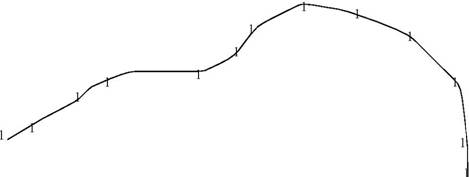
\includegraphics[width=\textwidth,height=\textheight/2,keepaspectratio=true]{modeling_data_image003.png}
\end{center}
\caption{Approximation of a B\+Spline from scattered points}
\end{DoxyImage}
 This class may be instantiated as follows\+: 
\begin{DoxyCode}
1 interp = GeomAPI\_Interpolate(points)
\end{DoxyCode}


From this object, the B\+Spline curve may be requested as follows\+: 
\begin{DoxyCode}
1 curve = interp.Curve()
\end{DoxyCode}


\subparagraph*{2D Approximation}

The class {\itshape Geom2d\+A\+P\+I\+\_\+\+Points\+To\+B\+Spline} allows building a 2\+D\+B\+Spline curve, which approximates a set of points. You have to define the lowest and highest degree of the curve, its continuity and a tolerance value for it.\+The tolerance value is used to check that points are not too close to each other, or tangential vectors not too small. The resulting B\+Spline curve will be\+C2 or second degree continuous, except where a tangency constraint is defined on a point through which the curve passes. In this case, it will be only C1continuous.

\subparagraph*{3D Approximation}

The class {\itshape Geom\+A\+P\+I\+\_\+\+Points\+To\+B\+Spline} allows building a 3D B\+Splinecurve, which approximates a set of points. It is necessary to define the lowest and highest degree of the curve, its continuity and tolerance. The tolerance value is used to check that points are not too close to each other,or that tangential vectors are not too small.

The resulting B\+Spline curve will be C2 or second degree continuous, except where a tangency constraint is defined on a point, through which the curve passes. In this case, it will be only C1 continuous. This class is instantiated as follows\+:


\begin{DoxyCode}
1 approx = GeomAPI\_PointsToBSpline(points, deg\_min, deg\_max, continuity, tol) 
\end{DoxyCode}


From this object, the B\+Spline curve may be requested as follows\+:


\begin{DoxyCode}
1 curve = approx.Curve()
\end{DoxyCode}


\subparagraph*{Surface Approximation}

The class {\itshape Geom\+A\+P\+I\+\_\+\+Points\+To\+B\+Spline\+Surface} allows building a B\+Spline surface, which approximates or interpolates a set of points.\hypertarget{occt_user_guides__modeling_data_occt_modat_1_1_3}{}\subsubsection{Advanced Approximation}\label{occt_user_guides__modeling_data_occt_modat_1_1_3}
Modules {\itshape App\+Def} and {\itshape App\+Par\+Curves} provide low-\/level functions, allowing more control over the approximations.

The low-\/level functions provide a second A\+PI with functions to\+:
\begin{DoxyItemize}
\item define compulsory tangents for an approximation. These tangents have origins and extremities,
\item approximate a set of curves in parallel to respect identical parameterization,
\item smooth approximations. This is to produce a faired curve.
\end{DoxyItemize}

You can also find functions to compute\+:
\begin{DoxyItemize}
\item the minimal box which includes a set of points,
\item the mean plane, line or point of a set of coplanar, collinear or coincident points.
\end{DoxyItemize}

\subparagraph*{Approximation by multiple point constraints}

{\itshape App\+Def} module provides low-\/level tools to allow parallel approximation of groups of points into Bezier or B-\/\+Spline curves using multiple point constraints.

The following low level services are provided\+:


\begin{DoxyItemize}
\item Definition of an array of point constraints\+:

The class {\itshape App\+Def\+\_\+\+Multi\+Line} allows defining a given number of multi-\/point constraints in order to build the multi-\/line, multiple lines passing through ordered multiple point constraints.

 
\begin{DoxyImage}
\begin{center}
 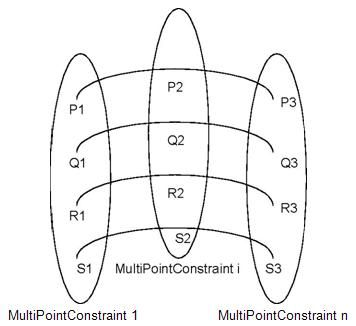
\includegraphics[width=\textwidth,height=\textheight/2,keepaspectratio=true]{modeling_data_image004.png}
\end{center}
\caption{Definition of a Multi\+Line using Multiple Point Constraints}
\end{DoxyImage}
 In this image\+:
\begin{DoxyItemize}
\item $Pi$, $Qi$, $Ri$ ... $Si$ can be 2D or 3D points,
\item defined as a group\+: $Pn$, $Qn$, $Rn$, ... $Sn$ form a Multipoint\+Constraint. They possess the same passage, tangency and curvature constraints,
\item $P1$, $P2$, ... $Pn$, or the $Q$, $R$, ... or $S$ series represent the lines to be approximated.
\end{DoxyItemize}
\item Definition of a set of point constraints\+:

The class {\itshape App\+Def\+\_\+\+Multi\+Point\+Constraint} allows defining a multiple point constraint and computing the approximation of sets of points to several curves.
\item Computation of an approximation of a Bezier curve from a set of points\+:

The class {\itshape App\+Def\+\_\+\+Compute} allows making an approximation of a set of points to a Bezier curve
\item Computation of an approximation of a B\+Spline curve from a set of points\+:

The class {\itshape App\+Def\+\_\+\+B\+Spline\+Compute} allows making an approximation of a set of points to a B\+Spline curve.
\item Definition of Variational Criteria\+:
\end{DoxyItemize}

The class {\itshape App\+Def\+\_\+\+Variational} allows fairing the approximation curve to a given number of points using a least squares method in conjunction with a variational criterion, usually the weights at each constraint point.

\subparagraph*{Approximation by parametric or geometric constraints}

{\itshape App\+Par\+Curves} module provides low-\/level tools to allow parallel approximation of groups of points into Bezier or B-\/\+Spline curve with parametric or geometric constraints, such as a requirement for the curve to pass through given points, or to have a given tangency or curvature at a particular point.

The algorithms used include\+:
\begin{DoxyItemize}
\item the least squares method,
\item a search for the best approximation within a given tolerance value.
\end{DoxyItemize}

The following low-\/level services are provided\+:


\begin{DoxyItemize}
\item Association of an index to an object\+:
\end{DoxyItemize}

The class {\itshape App\+Par\+Curves\+\_\+\+Constraint\+Couple} allows you associating an index to an object to compute faired curves using {\itshape App\+Def\+\_\+\+The\+Variational}.


\begin{DoxyItemize}
\item Definition of a set of approximations of Bezier curves\+:
\end{DoxyItemize}

The class {\itshape App\+Par\+Curves\+\_\+\+Multi\+Curve} allows defining the approximation of a multi-\/line made up of multiple Bezier curves.


\begin{DoxyItemize}
\item Definition of a set of approximations of B\+Spline curves\+:
\end{DoxyItemize}

The class {\itshape App\+Par\+Curves\+\_\+\+Multi\+B\+Sp\+Curve} allows defining the approximation of a multi-\/line made up of multiple B\+Spline curves.


\begin{DoxyItemize}
\item Definition of points making up a set of point constraints
\end{DoxyItemize}

The class {\itshape App\+Par\+Curves\+\_\+\+Multi\+Point} allows defining groups of 2D or 3D points making up a multi-\/line.

\subparagraph*{Example\+: How to approximate a curve with respect to tangency}

To approximate a curve with respect to tangency, follow these steps\+:


\begin{DoxyEnumerate}
\item Create an object of type {\itshape App\+Def\+\_\+\+Multi\+Point\+Constraints} from the set of points to approximate and use the method {\itshape Set\+Tang$\ast$to set the tangency vectors.}
\item {\itshape Create an object of type $\ast$\+App\+Def\+\_\+\+Multi\+Line$\ast$from the $\ast$\+App\+Def\+\_\+\+Multi\+Point\+Constraint}.
\item Use {\itshape App\+Def\+\_\+\+B\+Spline\+Compute}, which instantiates {\itshape Approx\+\_\+\+B\+Spline\+Compute\+Line} to perform the approximation.
\end{DoxyEnumerate}\hypertarget{occt_user_guides__modeling_data_occt_modat_1_2}{}\subsection{Direct Construction}\label{occt_user_guides__modeling_data_occt_modat_1_2}
Direct Construction methods from {\itshape gce}, {\itshape GC} and {\itshape G\+C\+E2d} modules provide simplified algorithms to build elementary geometric entities such as lines, circles and curves. They complement the reference definitions provided by the {\itshape gp}, {\itshape Geom} and {\itshape Geom2d} modules.

The algorithms implemented by {\itshape gce}, {\itshape G\+C\+E2d} and {\itshape GC} modules are simple\+: there is no creation of objects defined by advanced positional constraints (for more information on this subject, see {\itshape Geom2d\+Gcc} and {\itshape Gcc\+Ana}, which describe geometry by constraints).

For example, to construct a circle from a point and a radius using the {\itshape gp} module, it is necessary to construct axis {\itshape Ax2d} before creating the circle. If {\itshape gce} module is used, and {\itshape Ox} is taken for the axis, it is possible to create a circle directly from a point and a radius.

Another example is the class {\itshape gce\+\_\+\+Make\+Circ} providing a framework for defining eight problems encountered in the geometric construction of circles and implementing the eight related construction algorithms.

The object created (or implemented) is an algorithm which can be consulted to find out, in particular\+:


\begin{DoxyItemize}
\item its result, which is a {\itshape gp\+\_\+\+Circ},
\item its status. Here, the status indicates whether or not the construction was successful.
\end{DoxyItemize}

If it was unsuccessful, the status gives the reason for the failure.


\begin{DoxyCode}
1 p1 = gp\_Pnt(0., 0., 0.)
2 p2 = gp\_Pnt(0., 10., 0.)
3 p3 = gp\_Pnt(10., 0., 0.)
4 mc = gce\_MakeCirc(p1, p2, p3)
5 \textcolor{keywordflow}{if} mc.IsDone():
6   c = mc.Value()
\end{DoxyCode}


In addition, {\itshape gce}, {\itshape G\+C\+E2d} and {\itshape GC} each have a {\itshape Root} class, i.\+e. {\itshape gce\+\_\+\+Root}, {\itshape G\+C\+E\+\_\+\+Root} and {\itshape G\+C\+\_\+\+Root}. This class is the root of all classes in the module, which return a status. The returned status (successful construction or construction error) is described by the enumeration {\itshape gce\+\_\+\+Error\+Type}. Note, that classes, which construct geometric transformations do not return a status, and therefore do not inherit from {\itshape Root}.\hypertarget{occt_user_guides__modeling_data_occt_modat_1_2_1}{}\subsubsection{Non-\/persistent entities}\label{occt_user_guides__modeling_data_occt_modat_1_2_1}
The following algorithms used to build entities from non-\/persistent {\itshape gp} entities are provided by {\itshape gce} module.
\begin{DoxyItemize}
\item 2D line parallel to another at a distance,
\item 2D line parallel to another passing through a point,
\item 2D circle passing through two points,
\item 2D circle parallel to another at a distance,
\item 2D circle parallel to another passing through a point,
\item 2D circle passing through three points,
\item 2D circle from a center and a radius,
\item 2D hyperbola from five points,
\item 2D hyperbola from a center and two apexes,
\item 2D ellipse from five points,
\item 2D ellipse from a center and two apexes,
\item 2D parabola from three points,
\item 2D parabola from a center and an apex,
\item line parallel to another passing through a point,
\item line passing through two points,
\item circle coaxial to another passing through a point,
\item circle coaxial to another at a given distance,
\item circle passing through three points,
\item circle with its center, radius, and normal to the plane,
\item circle with its axis (center + normal),
\item hyperbola with its center and two apexes,
\item ellipse with its center and two apexes,
\item plane passing through three points,
\item plane from its normal,
\item plane parallel to another plane at a given distance,
\item plane parallel to another passing through a point,
\item plane from an array of points,
\item cylinder from a given axis and a given radius,
\item cylinder from a circular base,
\item cylinder from three points,
\item cylinder parallel to another cylinder at a given distance,
\item cylinder parallel to another cylinder passing through a point,
\item cone from four points,
\item cone from a given axis and two passing points,
\item cone from two points (an axis) and two radii,
\item cone parallel to another at a given distance,
\item cone parallel to another passing through a point,
\item all transformations (rotations, translations, mirrors,scaling transformations, etc.).
\end{DoxyItemize}

Each class from {\itshape gp} module, such as {\itshape gp\+\_\+\+Circ, gp\+\_\+\+Circ2d, gp\+\_\+\+Mirror, gp\+\_\+\+Mirror2d}, etc., has the corresponding {\itshape gce\+\_\+\+Make\+Circ, gce\+\_\+\+Make\+Circ2d, gce\+\_\+\+Make\+Mirror, gce\+\_\+\+Make\+Mirror2d}, etc. class from {\itshape gce} module.

It is possible to create a point using a {\itshape gce} module class, then question it to recover the corresponding {\itshape gp} object.


\begin{DoxyCode}
1 point1 = ... \textcolor{comment}{# any gp\_Pnt2d}
2 point2 = ... \textcolor{comment}{# any gp\_Pnt2d}
3 
4 l = gce\_MakeLin2d(point1, point2)
5 \textcolor{keywordflow}{if} l.Status() == gce\_Done:
6  l2d = l.Value() \textcolor{comment}{# returns a gp\_Lin2d}
\end{DoxyCode}
\hypertarget{occt_user_guides__modeling_data_occt_modat_1_2_2}{}\subsubsection{Persistent entities}\label{occt_user_guides__modeling_data_occt_modat_1_2_2}
{\itshape GC} and {\itshape G\+C\+E2d} modules provides an implementation of algorithms used to build entities from {\itshape Geom} and {\itshape Geom2D} modules. They implement the same algorithms as the {\itshape gce} module but create {\itshape persistent} entities, and also contain algorithms for trimmed surfaces and curves. The following algorithms are available\+:
\begin{DoxyItemize}
\item arc of a circle trimmed by two points,
\item arc of a circle trimmed by two parameters,
\item arc of a circle trimmed by one point and one parameter,
\item arc of an ellipse from an ellipse trimmed by two points,
\item arc of an ellipse from an ellipse trimmed by two parameters,
\item arc of an ellipse from an ellipse trimmed by one point and one parameter,
\item arc of a parabola from a parabola trimmed by two points,
\item arc of a parabola from a parabola trimmed by two parameters,
\item arc of a parabola from a parabola trimmed by one point and one parameter,
\item arc of a hyperbola from a hyperbola trimmed by two points,
\item arc of a hyperbola from a hyperbola trimmed by two parameters,
\item arc of a hyperbola from a hyperbola trimmed by one point and one parameter,
\item segment of a line from two points,
\item segment of a line from two parameters,
\item segment of a line from one point and one parameter,
\item trimmed cylinder from a circular base and a height,
\item trimmed cylinder from three points,
\item trimmed cylinder from an axis, a radius, and a height,
\item trimmed cone from four points,
\item trimmed cone from two points (an axis) and a radius,
\item trimmed cone from two coaxial circles.
\end{DoxyItemize}

Each class from {\itshape G\+C\+E2d} module, such as {\itshape G\+C\+E2d\+\_\+\+Circle, G\+C\+E2d\+\_\+\+Ellipse, G\+C\+E2d\+\_\+\+Mirror}, etc., has the corresponding {\itshape Geom2d\+\_\+\+Make\+Circle, Geom2d\+\_\+\+Make\+Ellipse, Geom2d\+\_\+\+Make\+Mirror}, etc. class from {\itshape Geom2d} module. Besides, the class {\itshape G\+C\+E2d\+\_\+\+Make\+Arc\+Of\+Circle} returns an object of type {\itshape Geom2d\+\_\+\+Trimmed\+Curve}.

Each class from {\itshape GC} module, such as {\itshape G\+C\+\_\+\+Circle, G\+C\+\_\+\+Ellipse, G\+C\+\_\+\+Mirror}, etc., has the corresponding {\itshape Geom\+\_\+\+Make\+Circle, Geom\+\_\+\+Make\+Ellipse, Geom\+\_\+\+Make\+Mirror}, etc. class from {\itshape Geom} module. The {\itshape Value} method for following classes return objects of type {\itshape Geom\+\_\+\+Trimmed\+Curve}\+:
\begin{DoxyItemize}
\item {\itshape G\+C\+\_\+\+Make\+Arc\+Of\+Circle}
\item {\itshape G\+C\+\_\+\+Make\+Arc\+Of\+Ellipse}
\item {\itshape G\+C\+\_\+\+Make\+Arc\+Of\+Hyperbola}
\item {\itshape G\+C\+\_\+\+Make\+Arc\+Of\+Parabola}
\item {\itshape G\+C\+\_\+\+Make\+Segment}
\end{DoxyItemize}\hypertarget{occt_user_guides__modeling_data_occt_modat_1_3}{}\subsection{Conversion to and from B\+Splines}\label{occt_user_guides__modeling_data_occt_modat_1_3}
The conversion to and from B\+Splines component has two distinct purposes\+:
\begin{DoxyItemize}
\item firstly, it provides a homogeneous formulation which can be used to describe any curve or surface. This is useful for writing algorithms for a single data structure model. The B\+Spline formulation can be used to represent most basic geometric objects provided by the components which describe geometric data structures (\char`\"{}\+Fundamental Geometry Types\char`\"{}, \char`\"{}2\+D Geometry Types\char`\"{} and \char`\"{}3\+D Geometry Types\char`\"{} components),
\item secondly, it can be used to divide a B\+Spline curve or surface into a series of curves or surfaces, thereby providing a higher degree of continuity. This is useful for writing algorithms which require a specific degree of continuity in the objects to which they are applied. Discontinuities are situated on the boundaries of objects only.
\end{DoxyItemize}

The \char`\"{}\+Conversion to and from B\+Splines\char`\"{} component is composed of three modules.

The {\itshape Convert} module provides algorithms to convert the following into a B\+Spline curve or surface\+:


\begin{DoxyItemize}
\item a bounded curve based on an elementary 2D curve (line, circle or conic) from the {\itshape gp} module,
\item a bounded surface based on an elementary surface (cylinder, cone, sphere or torus) from the {\itshape gp} module,
\item a series of adjacent 2D or 3D Bezier curves defined by their poles.
\end{DoxyItemize}

These algorithms compute the data needed to define the resulting B\+Spline curve or surface. This elementary data (degrees, periodic characteristics, poles and weights, knots and multiplicities) may then be used directly in an algorithm, or can be used to construct the curve or the surface by calling the appropriate constructor provided by the classes {\itshape Geom2d\+\_\+\+B\+Spline\+Curve, Geom\+\_\+\+B\+Spline\+Curve} or {\itshape Geom\+\_\+\+B\+Spline\+Surface}.

The {\itshape Geom2d\+Convert} module provides the following\+:


\begin{DoxyItemize}
\item a global function which is used to construct a B\+Spline curve from a bounded curve based on a 2D curve from the Geom2d module,
\item a splitting algorithm which computes the points at which a 2D B\+Spline curve should be cut in order to obtain arcs with the same degree of continuity,
\item global functions used to construct the B\+Spline curves created by this splitting algorithm, or by other types of segmentation of the B\+Spline curve,
\item an algorithm which converts a 2D B\+Spline curve into a series of adjacent Bezier curves.
\end{DoxyItemize}

The {\itshape Geom\+Convert} module also provides the following\+:


\begin{DoxyItemize}
\item a global function used to construct a B\+Spline curve from a bounded curve based on a curve from the Geom module,
\item a splitting algorithm, which computes the points at which a B\+Spline curve should be cut in order to obtain arcs with the same degree of continuity,
\item global functions to construct B\+Spline curves created by this splitting algorithm, or by other types of B\+Spline curve segmentation,
\item an algorithm, which converts a B\+Spline curve into a series of adjacent Bezier curves,
\item a global function to construct a B\+Spline surface from a bounded surface based on a surface from the Geom module,
\item a splitting algorithm, which determines the curves along which a B\+Spline surface should be cut in order to obtain patches with the same degree of continuity,
\item global functions to construct B\+Spline surfaces created by this splitting algorithm, or by other types of B\+Spline surface segmentation,
\item an algorithm, which converts a B\+Spline surface into a series of adjacent Bezier surfaces,
\item an algorithm, which converts a grid of adjacent Bezier surfaces into a B\+Spline surface.
\end{DoxyItemize}\hypertarget{occt_user_guides__modeling_data_occt_modat_1_4}{}\subsection{Points on Curves}\label{occt_user_guides__modeling_data_occt_modat_1_4}
The Points on Curves component comprises high level functions providing an A\+PI for complex algorithms that compute points on a 2D or 3D curve.

The following characteristic points exist on parameterized curves in 3d space\+:
\begin{DoxyItemize}
\item points equally spaced on a curve,
\item points distributed along a curve with equal chords,
\item a point at a given distance from another point on a curve.
\end{DoxyItemize}

{\itshape G\+C\+Pnts} module provides algorithms to calculate such points\+:
\begin{DoxyItemize}
\item {\itshape G\+C\+Pnts\+\_\+\+Abscissa\+Point} calculates a point on a curve at a given distance from another point on the curve.
\item {\itshape G\+C\+Pnts\+\_\+\+Uniform\+Abscissa} calculates a set of points at a given abscissa on a curve.
\item {\itshape G\+C\+Pnts\+\_\+\+Uniform\+Deflection} calculates a set of points at maximum constant deflection between the curve and the polygon that results from the computed points.
\end{DoxyItemize}

\subsubsection*{Example\+: Visualizing a curve.}

Let us take an adapted curve {\bfseries C}, i.\+e. an object which is an interface between the services provided by either a 2D curve from the module Geom2d (in case of an Adaptor\+\_\+\+Curve2d curve) or a 3D curve from the module Geom (in case of an Adaptor\+\_\+\+Curve curve), and the services required on the curve by the computation algorithm. The adapted curve is created in the following way\+:

{\itshape 2D case \+:} 
\begin{DoxyCode}
1 mycurve = some Handle\_Geom2d\_Curve
2 c = Geom2dAdaptor\_Curve(mycurve)
\end{DoxyCode}


{\itshape 3D case \+:} 
\begin{DoxyCode}
1 mycurve = some Handle\_Geom\_Curve 
2 c = GeomAdaptor\_Curve(mycurve) 
\end{DoxyCode}


The algorithm is then constructed with this object\+:


\begin{DoxyCode}
1 my\_algo = GCPnts\_UniformDeflection 
2 deflection = ... \textcolor{comment}{# any floar number}
3 my\_algo.Initialize(c, deflection)
4 \textcolor{keywordflow}{if} myAlgo.IsDone():
5   nbr = myAlgo.NbPoints()
6   \textcolor{keywordflow}{for} i \textcolor{keywordflow}{in} range(1, param): 
7     param = myAlgo.Parameter(i)
\end{DoxyCode}
\hypertarget{occt_user_guides__modeling_data_occt_modat_1_5}{}\subsection{Extrema}\label{occt_user_guides__modeling_data_occt_modat_1_5}
The classes to calculate the minimum distance between points, curves, and surfaces in 2d and 3d are provided by {\itshape Geom\+A\+PI} and {\itshape Geom2d\+A\+PI} modules.

These modules calculate the extrema of distance between\+:
\begin{DoxyItemize}
\item point and a curve,
\item point and a surface,
\item two curves,
\item a curve and a surface,
\item two surfaces.
\end{DoxyItemize}

\subsubsection*{Extrema between Curves}

The {\itshape Geom2d\+A\+P\+I\+\_\+\+Extrema\+Curve\+Curve} class allows calculation of all extrema between two 2D geometric curves. Extrema are the lengths of the segments orthogonal to two curves.

The {\itshape Geom\+A\+P\+I\+\_\+\+Extrema\+Curve\+Curve} class allows calculation of all extrema between two 3D geometric curves. Extrema are the lengths of the segments orthogonal to two curves.

\subsubsection*{Extrema between Curve and Surface}

The {\itshape Geom\+A\+P\+I\+\_\+\+Extrema\+Curve\+Surface} class allows calculation of all extrema between a 3D curve and a surface. Extrema are the lengths of the segments orthogonal to the curve and the surface.

\subsubsection*{Extrema between Surfaces}

The {\itshape Geom\+A\+P\+I\+\_\+\+Extrema\+Surface\+Surface} class allows calculation of all extrema between two surfaces. Extrema are the lengths of the segments orthogonal to two surfaces.\hypertarget{occt_user_guides__modeling_data_occt_modat_2}{}\section{2\+D Geometry}\label{occt_user_guides__modeling_data_occt_modat_2}
{\itshape Geom2d} module defines geometric objects in 2dspace. The objects are non-\/persistent and are handled by reference. In particular, {\itshape Geom2d} module provides classes for\+:
\begin{DoxyItemize}
\item description of points, vectors and curves,
\item their positioning in the plane using coordinate systems,
\item their geometric transformation, by applying translations, rotations, symmetries, scaling transformations and combinations thereof.
\end{DoxyItemize}

The following objects are available\+:
\begin{DoxyItemize}
\item point,
\item cartesian point,
\item vector,
\item direction,
\item vector with magnitude,
\item axis,
\item curve,
\item line,
\item conic\+: circle, ellipse, hyperbola, parabola,
\item rounded curve\+: trimmed curve, N\+U\+R\+BS curve, Bezier curve,
\item offset curve.
\end{DoxyItemize}

Before creating a geometric object, it is necessary to decide how the object is handled. The objects provided by {\itshape Geom2d} module are handled by reference rather than by value. Copying an instance copies the handle, not the object, so that a change to one instance is reflected in each occurrence of it. If a set of object instances is needed rather than a single object instance, {\itshape T\+Col\+Geom2d} module can be used. This module provides standard and frequently used instantiations of one-\/dimensional arrays and sequences for curves from {\itshape Geom2d} module. All objects are available in two versions\+:
\begin{DoxyItemize}
\item handled by reference,
\item handled by value.
\end{DoxyItemize}

The key characteristic of {\itshape Geom2d} curves is that they are parameterized. Each class provides functions to work with the parametric equation of the curve, and, in particular, to compute the point of parameter $u$ on a curve and the derivative vectors of order $1, 2.., N$ at this point.

As a consequence of the parameterization, a {\itshape Geom2d} curve is naturally oriented.

Parameterization and orientation differentiate elementary {\itshape Geom2d$\ast$curves from their equivalent as provided by $\ast$gp} module. {\itshape Geom2d} module provides conversion functions to transform a {\itshape Geom2d} object into a {\itshape gp} object, and vice-\/versa, when this is possible.

Moreover, {\itshape Geom2d} module provides more complex curves, including Bezier curves, B\+Spline curves, trimmed curves and offset curves.

{\itshape Geom2d} objects are organized according to an inheritance structure over several levels.

Thus, an ellipse (specific class {\itshape Geom2d\+\_\+\+Ellipse}) is also a conical curve and inherits from the abstract class {\itshape Geom2d\+\_\+\+Conic}, while a Bezier curve (concrete class {\itshape Geom2d\+\_\+\+Bezier\+Curve}) is also a bounded curve and inherits from the abstract class {\itshape Geom2d\+\_\+\+Bounded\+Curve}; both these examples are also curves (abstract class {\itshape Geom2d\+\_\+\+Curve}). Curves, points and vectors inherit from the abstract class$\ast$\+Geom2d\+\_\+\+Geometry,$\ast$ which describes the properties common to any geometric object from the {\itshape Geom2d} module.

This inheritance structure is open and it is possible to describe new objects, which inherit from those provided in the {\itshape Geom2d} module, provided that they respect the behavior of the classes from which they are to inherit.

Finally, {\itshape Geom2d} objects can be shared within more complex data structures. This is why they are used within topological data structures, for example.

{\itshape Geom2d} module uses the services of the {\itshape gp} module to\+:
\begin{DoxyItemize}
\item implement elementary algebraic calculus and basic analytic geometry,
\item describe geometric transformations which can be applied to {\itshape Geom2d} objects,
\item describe the elementary data structures of {\itshape Geom2d} objects.
\end{DoxyItemize}

However, the {\itshape Geom2d} module essentially provides data structures and not algorithms. You can refer to the {\itshape G\+C\+E2d} module to find more evolved construction algorithms for {\itshape Geom2d} objects.\hypertarget{occt_user_guides__modeling_data_occt_modat_3}{}\section{3\+D Geometry}\label{occt_user_guides__modeling_data_occt_modat_3}
The {\itshape Geom} module defines geometric objects in 3d space and contains all basic geometric transformations, such as identity, rotation, translation, mirroring, scale transformations, combinations of transformations, etc. as well as special functions depending on the reference definition of the geometric object (e.\+g. addition of a control point on a B-\/\+Spline curve,modification of a curve, etc.).

In particular, it provides classes for\+:
\begin{DoxyItemize}
\item description of points, vectors, curves and surfaces,
\item their positioning in 3D space using axis or coordinate systems,
\item their geometric transformation, by applying translations, rotations, symmetries, scaling transformations and combinations thereof.
\end{DoxyItemize}

The following non-\/persistent and reference-\/handled objects are available\+:
\begin{DoxyItemize}
\item point,
\item cartesian point,
\item vector,
\item direction,
\item vector with magnitude,
\item axis,
\item curve,
\item line,
\item conic\+: circle, ellipse, hyperbola, parabola,
\item offset curve,
\item elementary surface\+: plane, cylinder, cone, sphere, torus,
\item bounded curve\+: trimmed curve, N\+U\+R\+BS curve, Bezier curve,
\item bounded surface\+: rectangular trimmed surface, N\+U\+R\+BS surface, Bezier surface,
\item swept surface\+: surface of linear extrusion, surface of revolution,
\item offset surface.
\end{DoxyItemize}

The key characteristic of {\itshape Geom} curves and surfaces is that they are parameterized. Each class provides functions to work with the parametric equation of the curve or surface, and, in particular, to compute\+:
\begin{DoxyItemize}
\item the point of parameter $u$ on a curve, or
\item the point of parameters $(u, v)$ on a surface. together with the derivative vectors of order $1, 2, ... N$ at this point.
\end{DoxyItemize}

As a consequence of this parameterization, a Geom curve or surface is naturally oriented.

Parameterization and orientation differentiate elementary Geom curves and surfaces from the classes of the same (or similar) names found in {\itshape gp} module. {\itshape Geom} module also provides conversion functions to transform a Geom object into a {\itshape gp} object, and vice-\/versa, when such transformation is possible.

Moreover, $\ast$\+Geom$\ast$module provides more complex curves and surfaces, including\+:
\begin{DoxyItemize}
\item Bezier and B\+Spline curves and surfaces,
\item swept surfaces, for example surfaces of revolution and surfaces of linear extrusion,
\item trimmed curves and surfaces, and
\item offset curves and surfaces.
\end{DoxyItemize}

Geom objects are organized according to an inheritance structure over several levels. Thus, a sphere (concrete class {\itshape Geom\+\_\+\+Spherical\+Surface}) is also an elementary surface and inherits from the abstract class {\itshape Geom\+\_\+\+Elementary\+Surface}, while a Bezier surface (concrete class {\itshape Geom\+\_\+\+Bezier\+Surface}) is also a bounded surface and inherits from the abstract class {\itshape Geom\+\_\+\+Bounded\+Surface}; both these examples are also surfaces (abstract class {\itshape Geom\+\_\+\+Surface}). Curves, points and vectors inherit from the abstract class {\itshape Geom\+\_\+\+Geometry,} which describes the properties common to any geometric object from the {\itshape Geom} module.

This inheritance structure is open and it is possible to describe new objects, which inherit from those provided in the Geom module, on the condition that they respect the behavior of the classes from which they are to inherit.

Finally, Geom objects can be shared within more complex data structures. This is why they are used within topological data structures, for example.

If a set of object instances is needed rather than a single object instance, {\itshape T\+Col\+Geom} module can be used. This module provides instantiations of one-\/ and two-\/dimensional arrays and sequences for curves from {\itshape Geom} module. All objects are available in two versions\+:
\begin{DoxyItemize}
\item handled by reference and
\item handled by value.
\end{DoxyItemize}

The {\itshape Geom} module uses the services of the {\itshape gp} module to\+:
\begin{DoxyItemize}
\item implement elementary algebraic calculus and basic analytic geometry,
\item describe geometric transformations which can be applied to Geom objects,
\item describe the elementary data structures of Geom objects.
\end{DoxyItemize}

However, the Geom module essentially provides data structures, not algorithms.

You can refer to the {\itshape GC} module to find more evolved construction algorithms for Geom objects.\hypertarget{occt_user_guides__modeling_data_occt_modat_4}{}\section{Properties of Shapes}\label{occt_user_guides__modeling_data_occt_modat_4}
\hypertarget{occt_user_guides__modeling_data_occt_modat_4_1}{}\subsection{Local Properties of Shapes}\label{occt_user_guides__modeling_data_occt_modat_4_1}
{\itshape B\+Rep\+L\+Prop} module provides the Local Properties of Shapes component, which contains algorithms computing various local properties on edges and faces in a B\+Rep model.

The local properties which may be queried are\+:


\begin{DoxyItemize}
\item for a point of parameter $u$ on a curve which supports an edge \+:
\begin{DoxyItemize}
\item the point,
\item the derivative vectors, up to the third degree,
\item the tangent vector,
\item the normal,
\item the curvature, and the center of curvature;
\end{DoxyItemize}
\item for a point of parameter $(u, v)$ on a surface which supports a face \+:
\begin{DoxyItemize}
\item the point,
\item the derivative vectors, up to the second degree,
\item the tangent vectors to the $u$ and $v$ isoparametric curves,
\item the normal vector,
\item the minimum or maximum curvature, and the corresponding directions of curvature;
\end{DoxyItemize}
\item the degree of continuity of a curve which supports an edge, built by the concatenation of two other edges, at their junction point.
\end{DoxyItemize}

Analyzed edges and faces are described as {\itshape B\+Rep\+Adaptor} curves and surfaces, which provide shapes with an interface for the description of their geometric support. The base point for local properties is defined by its $u$ parameter value on a curve, or its $(u, v)$ parameter values on a surface.\hypertarget{occt_user_guides__modeling_data_occt_modat_4_2}{}\subsection{Local Properties of Curves and Surfaces}\label{occt_user_guides__modeling_data_occt_modat_4_2}
The \char`\"{}\+Local Properties of Curves and Surfaces\char`\"{} component provides algorithms for computing various local properties on a Geom curve (in 2D or 3D space) or a surface. It is composed of\+:


\begin{DoxyItemize}
\item {\itshape Geom2d\+L\+Prop} module, which allows computing Derivative and Tangent vectors (normal and curvature) of a parametric point on a 2D curve;
\item {\itshape Geom\+L\+Prop} module, which provides local properties on 3D curves and surfaces
\item {\itshape L\+Prop} module, which provides an enumeration used to characterize a particular point on a 2D curve.
\end{DoxyItemize}

Curves are either {\itshape Geom\+\_\+\+Curve} curves (in 3D space) or {\itshape Geom2d\+\_\+\+Curve} curves (in the plane). Surfaces are {\itshape Geom\+\_\+\+Surface} surfaces. The point on which local properties are calculated is defined by its u parameter value on a curve, and its $(u, v)$ parameter values on a surface.

It is possible to query the same local properties for points as mentioned above, and additionally for 2D curves\+:


\begin{DoxyItemize}
\item the points corresponding to a minimum or a maximum of curvature,
\item the inflection points.
\end{DoxyItemize}

\subparagraph*{Example\+: How to check the surface concavity}

To check the concavity of a surface, proceed as follows\+:


\begin{DoxyEnumerate}
\item sample the surface and compute at each point the Gaussian curvature.
\item if the value of the curvature changes of sign, the surface is concave or convex depending on the point of view.
\item to compute a Gaussian curvature, use the class {\itshape Geom\+L\+Prop\+\_\+\+S\+Lprops}, which instantiates the generic class {\itshape L\+Prop\+\_\+\+S\+L\+Props} and use the method {\itshape Gaussian\+Curvature}.
\end{DoxyEnumerate}\hypertarget{occt_user_guides__modeling_data_occt_modat_4_3}{}\subsection{Global Properties of Shapes}\label{occt_user_guides__modeling_data_occt_modat_4_3}
The Global Properties of Shapes component provides algorithms for computing the global properties of a composite geometric system in 3D space, and frameworks to query the computed results.

The global properties computed for a system are \+:
\begin{DoxyItemize}
\item mass,
\item mass center,
\item matrix of inertia,
\item moment about an axis,
\item radius of gyration about an axis,
\item principal properties of inertia such as principal axis, principal moments, and principal radius of gyration.
\end{DoxyItemize}

Geometric systems are generally defined as shapes. Depending on the way they are analyzed, these shapes will give properties of\+:


\begin{DoxyItemize}
\item lines induced from the edges of the shape,
\item surfaces induced from the faces of the shape,
\item volumes induced from the solid bounded by the shape.
\end{DoxyItemize}

The global properties of several systems may be brought together to give the global properties of the system composed of the sum of all individual systems.

The Global Properties of Shapes component is composed of\+:
\begin{DoxyItemize}
\item seven functions for computing global properties of a shape\+: one function for lines, two functions for surfaces and four functions for volumes. The choice of functions depends on input parameters and algorithms used for computation ({\itshape brepgprop\+\_\+$\ast$$\ast$ global functions),}
\item {\itshape a framework for computing global properties for a set of points ($\ast$\+G\+Prop\+\_\+\+P\+G\+Props}),
\item a general framework to bring together the global properties retained by several more elementary frameworks, and provide a general programming interface to consult computed global properties.
\end{DoxyItemize}

Modules {\itshape Geom\+L\+Prop} and {\itshape Geom2d\+L\+Prop} provide algorithms calculating the local properties of curves and surfaces

A curve (for one parameter) has the following local properties\+:
\begin{DoxyItemize}
\item point,
\item derivative,
\item tangent,
\item normal,
\item curvature,
\item center of curvature.
\end{DoxyItemize}

A surface (for two parameters $u$ and $v$) has the following local properties\+:
\begin{DoxyItemize}
\item point,
\item derivative (for $u$ and $v$),
\item tangent line (for $u$ and $v$),
\item normal,
\item max curvature,
\item min curvature,
\item main directions of curvature,
\item mean curvature,
\item gaussian curvature.
\end{DoxyItemize}

Among others, the following classes/methods are available\+:
\begin{DoxyItemize}
\item {\itshape Geom\+L\+Prop\+\_\+\+C\+L\+Props} -\/ calculates the local properties of a curve (tangency, curvature,normal),
\item {\itshape Geom2d\+L\+Prop\+\_\+\+Cur\+And\+Inf2d} -\/ calculates the maximum and minimum curvatures and the inflection points of 2d curves,
\item {\itshape Geom\+L\+Prop\+\_\+\+S\+L\+Props} -\/ calculates the local properties of a surface (tangency, the normal and curvature),
\item {\itshape Geom2d\+L\+Prop\+\_\+\+Curve2d\+Tool.\+Continuity} -\/ calculates regularity at the junction of two curves.
\end{DoxyItemize}

Note that the B-\/spline curve and surface are accepted but they are not cut into pieces of the desired continuity. It is the global continuity, which is seen.\hypertarget{occt_user_guides__modeling_data_occt_modat_4_4}{}\subsection{Adaptors for Curves and Surfaces}\label{occt_user_guides__modeling_data_occt_modat_4_4}
Some Python\+O\+CC general algorithms may work theoretically on numerous types of curves or surfaces.

To do this, they simply get the services required of the analyzed curve or surface through an interface so as to a single A\+PI, whatever the type of curve or surface. These interfaces are called adaptors.

For example, {\itshape Adaptor3d\+\_\+\+Curve} is the abstract class which provides the required services by an algorithm which uses any 3d curve.

{\itshape Geom\+Adaptor} module provides interfaces\+:
\begin{DoxyItemize}
\item on a Geom curve,
\item on a curve lying on a Geom surface,
\item on a Geom surface.
\end{DoxyItemize}

{\itshape Geom2d\+Adaptor} module provides interfaces \+:
\begin{DoxyItemize}
\item on a {\itshape Geom2d} curve.
\end{DoxyItemize}

{\itshape B\+Rep\+Adaptor} module provides interfaces\+:
\begin{DoxyItemize}
\item on a face,
\item on an edge.
\end{DoxyItemize}

When you write an algorithm which operates on geometric objects, use {\itshape Adaptor3d} (or {\itshape Adaptor2d}) objects. As a result, you can use the algorithm with any kind of object, if you provide for this object an interface derived from {\itshape Adaptor3d} or {\itshape Adaptor2d}. These interfaces are easy to use\+: simply create an adapted curve or surface from a {\itshape Geom2d} curve, and then use this adapted curve as an argument for the algorithm which requires it.\hypertarget{occt_user_guides__modeling_data_occt_modat_history}{}\section{History of this document\+:}\label{occt_user_guides__modeling_data_occt_modat_history}
january 2018\+: first public release -\/ tagged v0 


% Index
\newpage
\phantomsection
\addcontentsline{toc}{part}{Index}
\printindex\n
\end{document}

